
\section{Real time application using TRAMP}
\label{sec:streamer}
When we got this assignment we had to look at what we would implement in order to test the TRAMP platform. In the sample code there was implemented a simple chat program, so we decided to implement something that streamed a lot of data. There are several ways to do this; we could make a file sharing system, an audio streaming application (like Skype) or a video streaming application. We decided on looking into FFMPEG.

FFMPEG is a complete cross-platform solution to record, convert and stream video and audio. It is a free software licensed under the LGPL or GPL (dependent on the configuration), and is the leading multimedia framework today.\cite{FFMPEG-homepage}
FFMPEG provides tools for converting, streaming, playing and analyzing multimedia, as well as a full developers library with the possibility to create almost anything you want. Big projects such as QStream, VLC, GStreamer and Google Chrome has used the framework.

Due to time constraints we decided we did not have enough time to implement this framework. Instead we implemented a streamer that copied over one big file by chunking the big file into small bits, sending them and putting them back together on the other side. This will in our eyes show the capabilities of TRAMP just as well as a more sophisticated streamer like the FFMPEG solution we had planned.

\subsection{Our implementation}
\begin{figure*}[ht!]
\centering
 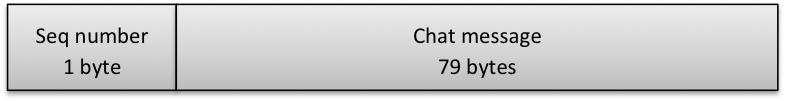
\includegraphics[width=300pt]{sendchatpkt.png}
 % sendchatpkt.png: 786x101 pixel, 150dpi, 13.31x1.71 cm, bb=0 0 377 48
\caption{Packet header for the chat application}
\label{Figure:Packet_header_chat}
\end{figure*}


\begin{figure*}[ht!]
\centering
 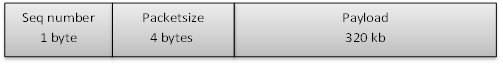
\includegraphics[width=300pt]{sendpkt.png}
 % sendchatpkt.png: 786x101 pixel, 150dpi, 13.31x1.71 cm, bb=0 0 377 48
\caption{Packet header for file chunks}
\label{Figure:pkt_header_file}
\end{figure*}

\begin{figure*}[ht!]
\centering
 
\includegraphics[width=300pt]{tramp_pkt.png}
 % sendchatpkt.png: 786x101 pixel, 150dpi, 13.31x1.71 cm, bb=0 0 377 48
\caption{TRAMP Daemon header}
\label{Figure:tramp_header}
\end{figure*}
Here we explain our implementation of a real time application using TRAMP framework. We use the example chat application provided as a basis for our application. We extend it to share files from producers to the consumers.
\begin{enumerate}
 \item \textbf{Producer}: We added a code snippet to read a given file from disk and push it to the shared memory which is detected by tramp daemon and sent to the connected consumers of the file subscribed with a label. For simplicity we use the same label ``ChatMSG'' provided in the example program to send the files as well. The files can be sent with the command

 \textbf{username$>$ send filename}

Before sending the file the producer sends a ``ChatMSG'' with the following format:
\textbf{file:filename|size}
Which helps consumer to expect file of \textbf{size} bytes to expect in the following packets. The producer reads the file in 320KB chunks. We extend the packet structure provided by chat application as shown in Figure \ref{Figure:Packet_header_chat} by adding a 4 byte size field for the payload size. The 320KB chunks along with sequence number (incremented for every new packet) and size of the payload as shown in Figure \ref{Figure:pkt_header_file} is written to the shared memory. Once the tramp daemon detects the change in header and reads the packet from shared memory and appends the header with message type and label to the packet as shown in Figure \ref{Figure:tramp_header}. Then the tram daemon writes the packet with the updated header to the socket connections with the consumers interested in this data.

\item \textbf{Consumer}: Consumer application is also extended version of chat program. Once the consumer a message starting with \textbf{file:} it prepares for receiving a file of specified size. The consumer continues to parse the size of the packet from the header and reads the specified size of bytes from packet and writes it to the disk. Once all the bytes are received the consumer closes the file and resumes normal chat operation. 
\end{enumerate}







